% ++++++++++++ Controller PSoC Master klassen ++++++++++++++
\subsubsection{Boundary-klasse: DistanceSensor} \label{sec:sw_design_distancesensor}

Denne klasse har til formål at styre kommunikation mellem Pi og afstandssensorerne, der er valgt at benytte I2C-kommunikation til dette. De 4 afstandssensorer er navngivet efter deres respektive placering på bilen: ''Front Left'' = ''FL'', ''Front Left'' = ''FL'' ''Front Left'' = ''RL'', ''Rear Right'' = ''RR'', herefter funktion  \texttt{getDistance("name")} kaldes udefra med navnet på den ønskede sensor som parameter, og afstanden returneres i cm. Afstandene gemmes i midlertidige variabler. Desuden skrives der til den globale Log ved klasseinitiering og klassenedlæggelse, samt ved eventuelle forekomster af fejl.

\begin{figure}[h]
\centering
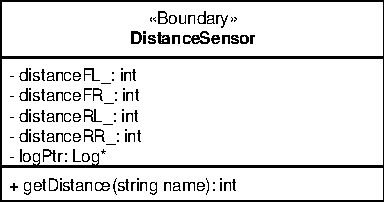
\includegraphics[]{../fig/diagrammer/bil/cd_distancesensor.pdf}
\caption{Klassebeskrivelse af boundary-klassen DistanceSensor}
\label{fig:cd_distancesensor}
\end{figure}

\textbf{Attributter}

\begin{table}[h]
	\begin{tabularx}{\textwidth}{| Z | Z | L{10cm} |} \hline
		Navn & Type & Beskrivelse \\\hline
		\texttt{distanceFL\_} & \texttt{int} 		& Midlertidig variabel der indeholder afstanden fra forreste venstre afstandssensor.\\\hline
		\texttt{distanceFR\_} & \texttt{int} 		& Midlertidig variabel der indeholder afstanden fra forreste højre afstandssensor.	\\\hline
		\texttt{distanceRL\_} & \texttt{int} 		& Midlertidig variabel der indeholder afstanden fra bagerste venstre afstandssensor \\\hline
		\texttt{distanceRR\_} & \texttt{int} 		& Midlertidig variabel der indeholder afstanden fra bagerste højre afstandssensor.	\\\hline
		\texttt{logPtr\_} 	 & \texttt{log*} 		& Pointer til at skrive i den globale Log											\\\hline
	\end{tabularx}
	\caption{Attributter for klassen DistanceSensor}
	\label{table:attr_distancesensor}
\end{table}
\clearpage

\textbf{Metoder}

\begin{table}[h]
	\begin{tabularx}{\textwidth}{| L{2.5 cm} | Z |} \hline
		Prototype 	& \texttt{int getDistance(string name)} \\\hline
		Parametre 	& \texttt{name} \newline Navnet på den sensor som der skal læses fra. Kan rumme én af fire muligheder "FL", "FR", "RL" og "RR". \\\hline
		Returværdi 	& \texttt{int} \newline Seneste afstandsmåling for den pågældende sensor. Værdien er angivet i cm. \\\hline
	\end{tabularx}
	\caption{Metodebeskrivelse for \texttt{getDistance}}
	\label{table:met_getdistance}
\end{table}
\clearpage